\documentclass[12pt]{article}

% fonts

\usepackage[T1]{fontenc}
\usepackage{newtxtext}
\usepackage{microtype}
\usepackage{bm}
\usepackage{amsthm} % before newtxmath b/c latex
\usepackage{newtxmath}
\usepackage[bb=ams,cal=cm]{mathalpha} % mt variants need MathTime Pro (not installed); matches template/preamble.tex

\usepackage{amsmath}
\usepackage{amsfonts}
\usepackage{thmtools}
\usepackage{mathtools}

% figures and tables

\usepackage{graphicx}
\usepackage{booktabs}

% spacing

\usepackage[parfill]{parskip}
\setlength{\parindent}{0pt}
\setlength{\parskip}{2ex plus 0.2ex minus 0.2ex}

% geometry of the page

\usepackage[
paper  = letterpaper,
left   = 1in,
right  = 1in,
top    = 1in,
bottom = 1in,
]{geometry}

% references

\usepackage[round]{natbib}
\usepackage[hidelinks]{hyperref}

% Generated by audited_analysis.py; MLE held-out results.
\newcommand{\auditN}{47{,}691}
\newcommand{\auditTrainN}{38{,}152}
\newcommand{\auditTestN}{9{,}539}
\newcommand{\auditGainSkew}{244.9}
\newcommand{\auditSeSkew}{48.1}
\newcommand{\auditGainSkewPerRunner}{0.0257}
\newcommand{\auditSeSkewPerRunner}{0.0050}
\newcommand{\auditGainGauss}{1151.5}
\newcommand{\auditSeGauss}{72.7}
\newcommand{\auditGainRaw}{108.6}
\newcommand{\auditSeRaw}{42.7}
\newcommand{\auditGainTen}{194.6}
\newcommand{\auditSeTen}{46.4}
\newcommand{\auditGainFifty}{280.8}
\newcommand{\auditSeFifty}{47.8}
\newcommand{\auditGainYearFourteen}{179.9}
\newcommand{\auditSeYearFourteen}{42.1}
\newcommand{\auditUnimodalGroups}{4}
\newcommand{\auditGroups}{4}


\usepackage{float}
\usepackage{tikz}
\usetikzlibrary{positioning,fit,arrows.meta}

% Tighten vertical spacing so each question fits the one-page limit.
% Fonts, 12pt size, and page geometry are left exactly as the template sets them.
\setlength{\parskip}{0.8ex plus 0.2ex minus 0.2ex}
\setlength{\abovedisplayskip}{3pt plus 1.5pt minus 1.5pt}
\setlength{\belowdisplayskip}{3pt plus 1.5pt minus 1.5pt}
\setlength{\abovedisplayshortskip}{3pt plus 1pt minus 1pt}
\setlength{\belowdisplayshortskip}{3pt plus 1pt minus 1pt}

\newcommand{\Norm}{\mathcal{N}}
\newcommand{\Dir}{\mathrm{Dirichlet}}
\newcommand{\sbeta}{\sqrt{1-\beta}}
\newcommand{\den}{\beta + (1-\beta)\tau_0^2}
\newcommand{\simplex}{\Delta_{V-1}}
\newcommand{\E}{\mathbb{E}}
\newcommand{\Var}{\mathrm{Var}}
\newcommand{\Cov}{\mathrm{Cov}}

\begin{document}

\begin{flushleft}
\textbf{Homework 1} \\
Jaisel Singh (js6897) \hfill October 16, 2026
\end{flushleft}

\textbf{Question 1: A First Look at Denoising Models}

\textit{(a) Posterior.} Both $p(x_0)$ and $p(x_1 \mid x_0)$ are Gaussian with mean
linear in $x_0$, so $(x_0, x_1)$ is jointly Gaussian and the posterior is Gaussian
before any algebra; the work is to find its two parameters. By Bayes' rule, keeping
only the factors that involve $x_0$,
\[
  p(x_0 \mid x_1) \;\propto\; p(x_0)\, p(x_1 \mid x_0)
  \;\propto\; \exp\left\{ -\frac{x_0^2}{2\tau_0^2}
  - \frac{(x_1 - \sbeta\, x_0)^2}{2\beta} \right\}.
\]
Expanding the square and dropping $x_1^2 / (2\beta)$, which is constant in $x_0$,
the exponent becomes
\[
  -\frac{x_0^2}{2\tau_0^2}
  - \frac{(1-\beta)\,x_0^2 - 2\sbeta\, x_0 x_1}{2\beta}
  \;=\; -\frac{1}{2}
  \underbrace{\left( \frac{1}{\tau_0^2} + \frac{1-\beta}{\beta} \right)}_{\textstyle \lambda}
  x_0^2
  \;+\; \underbrace{\frac{\sbeta\, x_1}{\beta}}_{\textstyle h}\, x_0 .
\]
Completing the square, any density proportional to
$\exp\{ -\tfrac12 \lambda x_0^2 + h x_0 \}$ is $\Norm(h/\lambda,\, 1/\lambda)$.
Here $\lambda = \big(\den\big) / (\beta \tau_0^2)$, so
\[
  \frac{1}{\lambda} = \frac{\beta\,\tau_0^2}{\den},
  \qquad
  \frac{h}{\lambda} = \frac{\sbeta\, x_1}{\beta} \cdot \frac{\beta\,\tau_0^2}{\den}
  = \frac{\sbeta\,\tau_0^2\, x_1}{\den},
\]
\[
  \boxed{\;
  x_0 \mid x_1 \;\sim\; \Norm\!\left(
  \frac{\sbeta\,\tau_0^2}{\den}\, x_1,\;\;
  \frac{\beta\,\tau_0^2}{\den}
  \right). \;}
\]
\textit{Check.} Jointly $\E[x_1] = 0$, $\Var(x_1) = (1-\beta)\tau_0^2 + \beta$ by total
variance, and $\Cov(x_0, x_1) = \E[x_0 \,\E(x_1 \mid x_0)] = \sbeta\,\tau_0^2$; Gaussian
conditioning, mean $\Cov(x_0,x_1)\,x_1 / \Var(x_1)$ and variance
$\tau_0^2 - \Cov(x_0,x_1)^2 / \Var(x_1)$, reproduces both boxed expressions.

The mean is $x_1 / \sbeta$, the inversion of the deterministic scaling, times
$(1-\beta)\tau_0^2 / \big((1-\beta)\tau_0^2 + \beta\big)$, the share of $\Var(x_1)$ due
to signal rather than injected noise; the posterior therefore shrinks that inversion
toward the prior mean $0$. Its variance is free of $x_1$: an observation relocates the
posterior without changing its spread.

\textit{(b) Limits.} As $\beta \to 0$ the mean tends to $x_1$ and the variance to $0$: the
step is the identity, so $x_1$ pins down $x_0$ exactly and the posterior is a point mass.
As $\beta \to 1$ the mean tends to $0$ and the variance to $\tau_0^2$: $x_1$ is pure noise,
the likelihood is independent of $x_0$, and the posterior falls back on the prior $\Norm(0, \tau_0^2)$.
Since $d\sigma^2/d\beta = \tau_0^4 / \big(\den\big)^2 > 0$, the variance climbs
monotonically between these limits, so $\beta$ sets how much of $x_0$ survives the step.

\textit{(c) Graphical model.} The statement describes one $(x_0, x_1)$ pair; the plate
shows i.i.d.\ replication over $N$ pairs (take $N=1$ here). Shaded $x_1^{(n)}$ is observed, $x_0^{(n)}$
is latent, and the fixed $\tau_0^2, \beta$ sit outside the plate, shared across all $n$.

\centerline{%
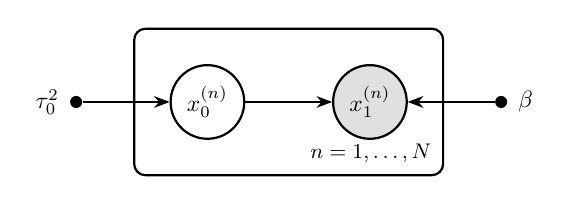
\begin{tikzpicture}[
    scale=0.85, transform shape,
    >={Stealth[length=2mm]},
    latent/.style = {circle, draw, thick, minimum size=11mm, inner sep=1pt},
    obs/.style    = {circle, draw, thick, fill=black!12, minimum size=11mm, inner sep=1pt},
    hyper/.style  = {circle, fill=black, minimum size=1.8mm, inner sep=0pt},
    node distance = 13mm
  ]
  \node[hyper, label={[label distance=1pt]left:$\tau_0^2$}] (tau) {};
  \node[latent, right=of tau] (x0) {$x_0^{(n)}$};
  \node[obs, right=of x0]     (x1) {$x_1^{(n)}$};
  \node[hyper, right=13mm of x1, label={[label distance=1pt]right:$\beta$}] (beta) {};

  \node[draw, thick, rounded corners, fit=(x0)(x1), inner sep=4.5mm] (plate) {};
  \node[anchor=south east, inner sep=1pt, font=\small]
       at ([shift={(-1.5mm,1.6mm)}]plate.south east) {$n = 1, \dots, N$};

  \draw[->] (tau) -- (x0);
  \draw[->] (x0)  -- (x1);
  \draw[->] (beta) -- (x1);
\end{tikzpicture}%
}

\newpage

\textbf{Question 2: Discrete Conjugacy}

\textit{(a) Posterior.} Write $\alpha_0 = \sum_{v=1}^V \alpha_v$ and
$B(\bm a) = \prod_{v=1}^V \Gamma(a_v) / \Gamma\big(\sum_{v=1}^V a_v\big)$, so the prior
density on the simplex $\simplex = \{\bm\pi : \pi_v \ge 0,\, \sum_v \pi_v = 1\}$ is
$p(\bm\pi) = B(\bm\alpha)^{-1} \prod_{v=1}^V \pi_v^{\alpha_v - 1}$; equivalently
$\int_{\simplex} \prod_{v=1}^V \pi_v^{a_v - 1} \, d\bm\pi = B(\bm a)$ for any $\bm a$ with
positive entries, an identity reused in part~(b). The likelihood is where the counts appear.
Writing one categorical draw as
$p(y_i \mid \bm\pi) = \pi_{y_i} = \prod_{v=1}^V \pi_v^{\mathbf{1}\{y_i = v\}}$ and
using conditional independence given $\bm\pi$,
\[
  p(y_1, \dots, y_n \mid \bm\pi)
  = \prod_{i=1}^n \prod_{v=1}^V \pi_v^{\mathbf{1}\{y_i = v\}}
  = \prod_{v=1}^V \pi_v^{\sum_{i=1}^n \mathbf{1}\{y_i = v\}}
  = \prod_{v=1}^V \pi_v^{n_v},
\]
so the data enter only through the counts $(n_1, \dots, n_V)$, a sufficient statistic,
and the likelihood is a product of powers of the $\pi_v$, matching the functional form
of the prior. That is exactly why the family is closed under conditioning. Multiplying,
\[
  p(\bm\pi \mid y_1, \dots, y_n)
  \;\propto\; \prod_{v=1}^V \pi_v^{\alpha_v - 1} \prod_{v=1}^V \pi_v^{n_v}
  \;=\; \prod_{v=1}^V \pi_v^{(\alpha_v + n_v) - 1}.
\]
The right side is the Dirichlet kernel with parameters $\alpha_v + n_v > 0$; a density is
pinned down by its kernel, so the normalizer is $B(\bm\alpha + \bm n)^{-1}$ and
\[
  \boxed{\; \bm\pi \mid y_1, \dots, y_n \;\sim\; \Dir(\alpha_1 + n_1, \,\dots,\, \alpha_V + n_V). \;}
\]
The prior parameters behave as pseudocounts: the data simply add $n_v$ to
$\alpha_v$, and the concentration grows from $\alpha_0$ to $\alpha_0 + n$.

\textit{(b) Posterior predictive.} Let $\bm\alpha' = \bm\alpha + \bm n$, so
$\alpha_0' = \sum_u \alpha_u' = \alpha_0 + n$. Given $\bm\pi$ the next draw is independent
of the previous ones, so conditioning on $\bm\pi$ and marginalizing it out,
\[
  p(y_{n+1} = v \mid y_{1:n})
  = \int_{\simplex} \pi_v \, p(\bm\pi \mid y_{1:n}) \, d\bm\pi
  = \E[\pi_v \mid y_{1:n}],
\]
the posterior mean of $\pi_v$. The extra factor of $\pi_v$ raises the $v$-th exponent by
one, replacing $\bm\alpha'$ with $\bm\alpha' + \bm e_v$, so that same identity applies:
\[
  \E[\pi_v \mid y_{1:n}]
  = \frac{1}{B(\bm\alpha')} \int_{\simplex} \prod_{u=1}^V \pi_u^{(\alpha_u' + \mathbf{1}\{u = v\}) - 1} \, d\bm\pi
  = \frac{B(\bm\alpha' + \bm e_v)}{B(\bm\alpha')}
  = \frac{\Gamma(\alpha_v' + 1)}{\Gamma(\alpha_v')} \cdot \frac{\Gamma(\alpha_0')}{\Gamma(\alpha_0' + 1)}
  = \frac{\alpha_v'}{\alpha_0'},
\]
where the $u \neq v$ factors cancel and $\Gamma(z+1) = z\,\Gamma(z)$ is used twice.
Hence
\[
  \boxed{\; p(y_{n+1} = v \mid y_1, \dots, y_n) = \frac{\alpha_v + n_v}{\alpha_0 + n},
  \qquad \alpha_0 = \sum_{u=1}^V \alpha_u. \;}
\]
These sum to one over $v$, since $\sum_v (\alpha_v + n_v) = \alpha_0 + n$. For $n>0$,
\vspace{-1ex}
\[
  \frac{\alpha_v + n_v}{\alpha_0 + n}
  = \frac{n}{\alpha_0 + n} \cdot \frac{n_v}{n}
  \;+\; \frac{\alpha_0}{\alpha_0 + n} \cdot \frac{\alpha_v}{\alpha_0}
\]
exhibits it as a convex combination of the maximum likelihood estimate $n_v / n$ and the
prior mean $\alpha_v / \alpha_0$, with $\alpha_0$ an effective prior sample size: it tends
to the MLE as $n \to \infty$ but keeps positive mass on every category even when
$n_v = 0$. This is additive smoothing, which becomes Laplace smoothing when $\alpha_v = 1$.


% >>> Q3 BEGIN (audited analysis)
\clearpage
\textbf{Question 3: Box's Loop}

{\small
\setlength{\parskip}{0.55ex plus 0.1ex minus 0.1ex}

\textit{(1) Question.} Among the available Boston Marathon race records, does a
two-component Gaussian mixture predict late-race slowing better than a single
Gaussian or a single skew-normal, and would that justify calling its components
``wall'' and ``no wall''? These are separate questions: a useful density
approximation need not identify two physiological states.

\textit{(2) Data and processing.} I use the public
\href{https://github.com/llimllib/bostonmarathon}{\textnormal{llimllib/bostonmarathon}}
scrape of BAA results. Its scraper retrieves
individual race-result pages and exports cumulative checkpoint times in minutes,
rounded to two decimals. The 2013 and 2014 files contain 16,164 and 31,984 rows;
variables include bib, recorded sex, age, and times at 5, 10, 20, 21.0975, 25, 30,
35, 40 and 42.195\,km. A row is a race performance, not necessarily a distinct
person across years; the exported files omit the 15\,km split.

I remove 105 wheelchair records, seven repeated bibs within a year, and 41 records
with an available segment pace outside the screening range 2--20\,min/km.
Missing tokens and nonpositive times become missing; non-increasing cumulative
times would also be blanked (none occur here). The loader interpolates isolated
interior gaps, but the analysis requires all four defining endpoints to be
observed, excluding another 304 records: \auditN{} remain, 457 fewer than the raw
files. A missing split's cause is unknown, and the slow-pace cutoff can remove a
real stop, so these are selection decisions rather than proof of faulty timing.

For cumulative time $T_d$ at distance $d$, define
\[
 a_i=\frac{T_{25,i}-T_{10,i}}{15},\qquad
 r_i=\log\!\left(\frac{(T_{40,i}-T_{30,i})/10}{a_i}\right),\qquad
 y_i=r_i-\widehat q_{.25}(a_i).
\]
Here $a_i$ is baseline pace and $r_i>0$ means the 30--40\,km window was slower.
Negative $y_i$ means less slowing than the reference, not necessarily a faster
late pace. The reference is the training sample's 25th percentile of $r$ in 40 baseline-pace
bins, interpolated between bin medians and held constant beyond them.
Figure~\ref{fig:audit-wall}a explores the raw relationship; panels b--c show the
centered distributions. This is empirical centering, \emph{not} a terrain
correction: the 30--40\,km window still includes Heartbreak Hill
(\href{https://www.baa.org/wp-content/uploads/docs/2025-03/129thBM_SpectatorGuide.pdf}{BAA course map}).
Pace reflects strategy and fatigue as well as ability, and shifting different
pace strata can change the pooled shape.

\textit{(3) Scope and limitations, set before the refit.} These records can assess
density fit in the observed sample, but contain no direct observation of glycogen
depletion, fueling, pain or perceived exhaustion. The source excludes
nonfinishers and acknowledges missing finishers; the 2013 race interruption adds
severe selection, so neither a population wall rate nor a lower bound on it is
identified. Boston's entry rules and course further limit generalization.
Nonfinisher splits and independently collected fueling, heart-rate and exhaustion
records would help distinguish timing patterns from a physiological event.

\textit{(4) Model and fitting.} For each recorded-sex $\times$ year group $g$, I fit
$\mathcal M_0:\ y_i\sim\Norm(\mu_g,\sigma_g^2)$, a single skew-normal $\mathcal M_s$,
and the latent-class model
\[
 z_i\sim\mathrm{Bernoulli}(\pi_g),\qquad
 y_i\mid z_i=k\sim\Norm(\mu_{k,g},\sigma_{k,g}^2),\quad \mu_{0,g}<\mu_{1,g}.
\]
I split records 80/20 within groups (seed 20261016; \auditTrainN{} training,
\auditTestN{} held out), estimate the reference only on training records, and fit
by maximum likelihood: closed form for $\mathcal M_0$, six-start numerical
optimization for $\mathcal M_s$, and six-start EM for the mixture, alternating
probabilistic component assignments with weighted parameter updates.
To prevent the mixture's unbounded likelihood at a collapsed component, each
standard deviation is constrained to at least $\max(10^{-4},0.02s_g)$, where
$s_g$ is the training standard deviation; all selected fits converge and none
uses that floor.

\newpage
\textit{(5) Results and criticism.} For each held-out record I compute
$d_i=\log\widehat p_2(y_i)-\log\widehat p_s(y_i)$; positive values favor the
mixture. The table reports $\sum_i d_i$ with approximate standard error
$\sqrt{\sum_g n_g s_{d,g}^2}$, respecting fixed group counts, treating records
as independent and holding the
trained fits fixed. These errors do not include training-set uncertainty,
repeat-runner dependence or variation across races.

\begin{center}
\begin{tabular}{lrr}
\toprule
Reference & Mixture minus skew-normal (nats) & Standard error \\
\midrule
25th percentile (primary) & \auditGainSkew & \auditSeSkew \\
None (raw log ratio) & \auditGainRaw & \auditSeRaw \\
10th percentile & \auditGainTen & \auditSeTen \\
50th percentile & \auditGainFifty & \auditSeFifty \\
\bottomrule
\end{tabular}
\end{center}

\begin{figure}[H]
\centering
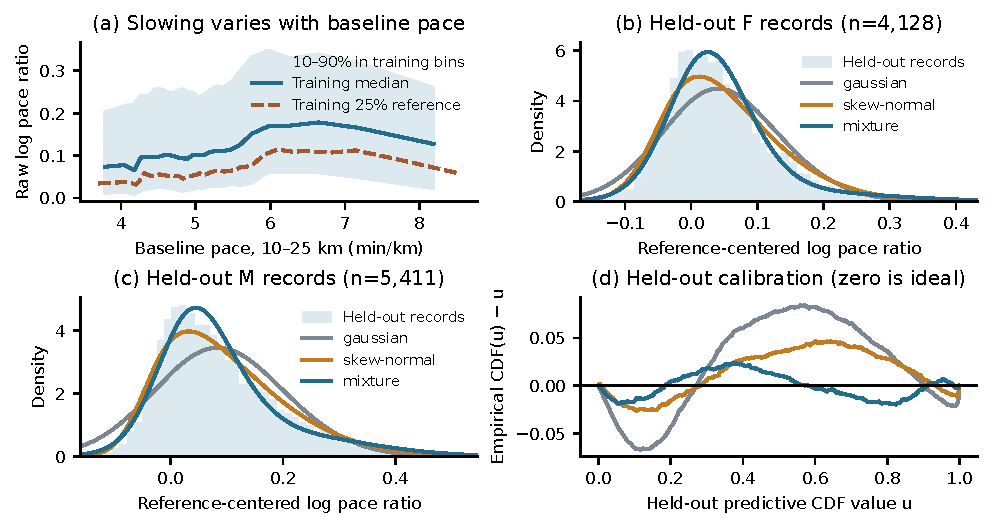
\includegraphics[width=\textwidth]{figures/audit_wall}
\caption{\small (a) Training quantiles; (b--c) held-out histograms and fitted densities,
zoomed to the bulk; (d) predictive-CDF calibration, where zero is ideal. Scores
include all tails; the mixture still shows misfit.}
\label{fig:audit-wall}
\end{figure}

The primary gain is \auditGainSkewPerRunner{} nats per record over the
skew-normal, and \auditGainGauss{} total nats (s.e.\ \auditSeGauss) over the
Gaussian. The advantage persists across references and in the 2014 held-out
subset (\auditGainYearFourteen{} nats, s.e.\ \auditSeYearFourteen{}, using the shared
training reference). Yet all \auditGroups{} fitted group mixture densities have
only \emph{one} mode on a dense grid. Their higher-mean components are wider and
dominate both extreme tails, including negative $y$, so component membership does
not identify a directional slowdown. The mixture improves these density
approximations; it establishes neither two biological regimes nor wall prevalence.
A skew-normal is only one possible unimodal alternative.

\textit{(6) Next step.} I would compare segment trajectories with independently
recorded exhaustion onset in a new, uninterrupted race, including nonfinishers.
The refined question is whether an abrupt, sustained slowdown coincides with that
observation after accounting for course location and initial pacing. This tests
what the latent label means. The current split is an internal diagnostic:
an earlier draft explored these data, and the sensitivity rows reuse the test
set, so neither is independent confirmation.

} % end small
% <<< Q3 END

\end{document}

%%% Local Variables:
%%% mode: latex
%%% TeX-master: t
%%% End:
